% =====================================================================================================
% Monitoring and improving the FAIRness of EarthPortal semantic artefacts: first conclusions
% Emmanuel Nyandu Kagarabi, CNRS / Data Terra, team meeting of 9 October 2026
% Compile with pdflatex (twice), e.g.  latexmk -pdf emmanuel_dataTerra_Slides_2026-10-09.tex
% =====================================================================================================
\documentclass[aspectratio=169,10pt]{beamer}

\usetheme[progressbar=foot, numbering=fraction, block=fill, sectionpage=progressbar]{metropolis}
\usepackage[T1]{fontenc}
\usepackage[utf8]{inputenc}
\usepackage[scaled=0.95]{helvet}
\usepackage{courier}
\usefonttheme[onlymath]{serif}
\usepackage{amsmath}
\usepackage{booktabs}
\usepackage{tabularx}
\usepackage{xcolor}
\usepackage{tikz}
\usetikzlibrary{arrows.meta, positioning, fit, calc, shapes.misc}
\usepackage{qrcode}
\usepackage{hyperref}

% ---- Colours of the Data Terra reports (dataterra-report.sty) ---------------------------------------
\definecolor{dtnavy}{HTML}{22245C}
\definecolor{dtblue}{HTML}{0B4F6C}
\definecolor{dtteal}{HTML}{1B7F5C}
\definecolor{dtindigo}{HTML}{5A5DB4}
\definecolor{dtred}{HTML}{A4303F}
\definecolor{dtamber}{HTML}{9A6A00}
\definecolor{dtband}{HTML}{EDF1F4}
\definecolor{dtgrey}{HTML}{5A6672}
\definecolor{dtink}{HTML}{1E2430}

\setbeamercolor{normal text}{fg=dtink, bg=white}
\setbeamercolor{frametitle}{fg=white, bg=dtnavy}
\setbeamercolor{title}{fg=dtnavy}
\setbeamercolor{subtitle}{fg=dtteal}
\setbeamercolor{progress bar}{fg=dtteal, bg=dtband}
\setbeamercolor{alerted text}{fg=dtred}
\setbeamercolor{example text}{fg=dtteal}
\setbeamercolor{block title}{fg=white, bg=dtnavy}
\setbeamercolor{block body}{fg=dtink, bg=dtband}
\setbeamercolor{block title alerted}{fg=white, bg=dtred}
\setbeamercolor{block body alerted}{fg=dtink, bg=dtband}
\setbeamercolor{block title example}{fg=white, bg=dtteal}
\setbeamercolor{block body example}{fg=dtink, bg=dtband}
\setbeamercolor{background canvas}{bg=white}
\setbeamertemplate{itemize item}{\color{dtteal}$\blacktriangleright$}
\setbeamertemplate{itemize subitem}{\color{dtgrey}\textbullet}
\setbeamerfont{frametitle}{size=\large}
\setbeamerfont{footnote}{size=\tiny}

% ---- Small helpers -----------------------------------------------------------------------------------
% A dashed placeholder telling which screenshot to take and paste here
\newcommand{\screenshot}[3]{%
  \begin{tikzpicture}
    \node[draw=dtteal, dashed, line width=0.9pt, rounded corners=4pt, fill=dtband,
          minimum width=#1, minimum height=#2, text width=#1-14pt, align=center, font=\scriptsize]
         {\textcolor{dtteal}{\textbf{SCREENSHOT TO PASTE HERE}}\\[3pt]#3};
  \end{tikzpicture}}
\newcommand{\evidence}[1]{{\scriptsize\color{dtgrey}#1}}
\newcommand{\nb}[1]{\textbf{\textcolor{dtteal}{#1}}}
\newcommand{\code}[1]{{\color{dtblue}\texttt{#1}}}
\newcommand{\bignum}[2]{{\color{#2}\fontsize{26}{28}\selectfont\bfseries #1}}

% ---- Title page --------------------------------------------------------------------------------------
\title{Monitoring and improving the FAIRness\\of EarthPortal semantic artefacts}
\subtitle{First conclusions: five notebooks, one audit per ontology, and what we learned about O'FAIRe}
\author{Emmanuel Nyandu Kagarabi}
\institute{\href{https://emmanuelnyandukagarabi.github.io/}{https://emmanuelnyandukagarabi.github.io/}\\Internship CNRS / Data Terra\\
           Supervisor: Christelle Pierkot }
\date{Montpellier, 9 October 2026}

\begin{document}

% =====================================================================================================
\begin{frame}[plain]
  \vspace{0.5cm}
  {\color{dtnavy}\LARGE\bfseries Monitoring and improving the FAIRness\\[2pt] of EarthPortal semantic artefacts\par}
  \vspace{6pt}
  {\color{dtteal}\large First conclusions: five notebooks, one audit per ontology,\\ and what we learned about O'FAIRe\par}
  \vspace{4pt}
  {\color{dtteal}\rule{\textwidth}{0.8pt}}
  \vspace{8pt}

  {\large\bfseries Emmanuel Nyandu Kagarabi}\\
  {\footnotesize Bac+5 (Maths) $\rightarrow$ MSc (AI4Science) $\rightarrow$ Master (DMC) : \href{https://emmanuelnyandukagarabi.github.io/}{https://emmanuelnyandukagarabi.github.io/}}\\
  {\small Internship CNRS / Data Terra\\
   Supervisor: Christelle Pierkot}\\
  {\small\color{dtgrey} Montpellier, 9 October 2026}
  \vfill
  \hfill
  
\includegraphics[height=0.8cm]{Figures/Logo_CNRS-fr.png}\hspace{0.5cm}
  
\includegraphics[height=0.8cm]{Figures/Logo_DATATERRA-fr.jpg}\hspace{0.5cm}
  
\includegraphics[height=1.15cm]{Figures/Logo_SISSA-it.png}
\end{frame}

% -----------------------------------------------------------------------------------------------------
\begin{frame}{Today in 30 minutes}
  \begin{columns}[T]
    \begin{column}{0.48\textwidth}
      \begin{enumerate}
        \item \textbf{Where I am} in the internship
        \item \textbf{O'FAIRe in five minutes}: what it measures, and how we read it
        \item \textbf{The pipeline}: five notebooks, from the API to one audit per ontology
        \item \textbf{What we found}: in the catalogue, and about O'FAIRe, with evidence
        \item \textbf{Environment and next steps}
      \end{enumerate}
    \end{column}
    \begin{column}{0.48\textwidth}
      \begin{exampleblock}{The one message of this talk}
        We use O'FAIRe as a \textbf{measuring instrument} to monitor and improve the FAIRness of the
        artefacts hosted on EarthPortal.\\[4pt]
        We do \textbf{not} change its implementation: improving O'FAIRe is another project, for
        someone else. But to read its scores correctly, we had to understand exactly how it
        computes them.
      \end{exampleblock}
    \end{column}
  \end{columns}
\end{frame}

% -----------------------------------------------------------------------------------------------------
\begin{frame}{Where I am in the internship}
  \small
  \begin{tabularx}{\textwidth}{@{}l X l@{}}
    \toprule
    \textbf{Task} & \textbf{What exists today} & \textbf{Status}\\
    \midrule
    1. Metadata guideline & Quick reference table (cheatsheet) of the 99 attributes, typos corrected
                          (Report 1); a \textbf{machine-readable} version generated from it & first version\\
    2. Audit of all artefacts & 92 audits, one per catalogue entry, with ranked actions & first run\\
    3. Towards automation & 5 notebooks, reproducible on any dated snapshot of the catalogue & manual run\\
    4. FAIR metrics & O'FAIRe questions, properties and Java implementation documented (Reports 2 to 4);
                      FOOPS! not studied yet & in progress\\
    \bottomrule
  \end{tabularx}
  \vfill
  \evidence{All code, tables, audits and reports:
    \href{https://github.com/EarthPortal/SA_Management}{github.com/EarthPortal/SA\_Management}
    (folders \code{docs/} and \code{earthportal\_sa\_audit/}).}
\end{frame}

% -----------------------------------------------------------------------------------------------------
\begin{frame}{EarthPortal on 8 October 2026, in numbers}
  \begin{columns}[T]
    \begin{column}{0.30\textwidth}
      \centering
      \bignum{92}{dtnavy}\\[-2pt]
      {\small public catalogue entries}\\[8pt]
      \begin{tabular}{@{}r l@{}}
        \textbf{\textcolor{dtteal}{68}} & artefacts\\
        \textbf{\textcolor{dtindigo}{19}} & views\\
        \textbf{\textcolor{dtgrey}{5}} & metadata-only records\\
      \end{tabular}
    \end{column}
    \begin{column}{0.30\textwidth}
      \centering
      \bignum{130}{dtnavy}\\[-2pt]
      {\small metadata fields stored by the portal}\\[8pt]
      \begin{tabular}{@{}r l@{}}
        110 & on each submission\\
        20 & on the ontology record\\
      \end{tabular}
    \end{column}
    \begin{column}{0.34\textwidth}
      \centering
      \bignum{99}{dtnavy}\\[-2pt]
      {\small attributes in the Metadata guideline}\\[8pt]
      \begin{tabular}{@{}r l@{}}
        20 & Mandatory\\
        58 & Recommended\\
        21 & Optional\\
      \end{tabular}
    \end{column}
  \end{columns}
  \vfill
  \begin{alertblock}{The catalogue moves: why every result carries a date}
    Between 6 and 8 October, \code{OSO-DCAT} and \code{OSO-VOID} became \textbf{views of OSO},
    \code{OSO-SHACL} appeared as a new view, and \code{SCHEMA-ORG} left the public catalogue
    (71 / 16 / 5 became 68 / 19 / 5).
    Our pipeline works on \textbf{dated snapshots}, so each run can be reproduced and compared.
  \end{alertblock}
\end{frame}

% =====================================================================================================
\section{O'FAIRe in five minutes}

% -----------------------------------------------------------------------------------------------------
\begin{frame}{What is O'FAIRe?}
  \begin{columns}[T]
    \begin{column}{0.52\textwidth}
      \small
      \textbf{O'FAIRe} (\emph{Ontology FAIRness Evaluator}) scores how FAIR a semantic artefact is,
      from \textbf{its metadata record} on an OntoPortal instance (AgroPortal, EarthPortal, \dots).
      \begin{itemize}
        \item 4 principles $\rightarrow$ 15 sub-principles $\rightarrow$ \textbf{61 questions}
        \item each question pays credits on a ladder, from 0 to its maximum $m_q$
        \item fully automatic: the metadata held by the portal, plus a few live checks (do the URLs resolve?)
      \end{itemize}
      \vspace{2pt}
      \scriptsize
      \begin{tabular}{@{}l c c c c | c@{}}
        \toprule
        & F & A & I & R & \textbf{Total}\\
        \midrule
        Questions & 13 & 13 & 15 & 20 & \textbf{61}\\
        Maximum & 113 & 113 & 109 & 143 & \textbf{478}\\
        \bottomrule
      \end{tabular}
    \end{column}
    \begin{column}{0.45\textwidth}
      \begin{block}{The score of an artefact $o$}
        \vspace{-6pt}
        \[
          S(o) = \sum_{q=1}^{61} s_q(o), \qquad 0 \le s_q(o) \le m_q
        \]
        \vspace{-4pt}
        \[
          N(o) = \left\lfloor 100 \cdot \frac{S(o)}{478} \right\rfloor
        \]
        {\scriptsize 478: the sum of the maxima of the 15 sub-principles.}
      \end{block}
      {\small\textbf{Example, OSO:} $S = 364.36$, so $N = \lfloor 76.2 \rfloor = 76$.}\\[6pt]
      \evidence{Amdouni, Bouazzouni \& Jonquet (2022), \emph{O'FAIRe makes you an offer: metadata-based
      automatic FAIRness assessment for ontologies and semantic resources}, IJMSO 16(1).}
    \end{column}
  \end{columns}
\end{frame}

% -----------------------------------------------------------------------------------------------------
\begin{frame}{How we use it: an instrument, not an object of study}
  \begin{columns}[c]
    \begin{column}{0.55\textwidth}
      \begin{exampleblock}{What we do}
        \begin{itemize}
          \item take O'FAIRe's answers \textbf{as they are}, for every entry of the catalogue
          \item link each question to the guideline attributes it reads
          \item turn the lost points into \textbf{curation actions} for authors, curators and the portal
          \item follow the scores over time, snapshot after snapshot
        \end{itemize}
      \end{exampleblock}
    \end{column}
    \begin{column}{0.42\textwidth}
      \begin{alertblock}{What we do not do}
        Modify, fork or re-implement O'FAIRe. Its improvement is a separate project.
      \end{alertblock}
      \vspace{4pt}
      \begin{block}{But we had to read the code}
        {\small To tell a real 0 from a question that measures nothing, we read the Java source
        (\code{agroportal/fairness}, commit \code{24def6b}, 4 June 2026) and checked every claim on
        the EarthPortal data.}
      \end{block}
    \end{column}
  \end{columns}
\end{frame}

% -----------------------------------------------------------------------------------------------------
\begin{frame}{What the 478 points measure on EarthPortal}
  \centering
  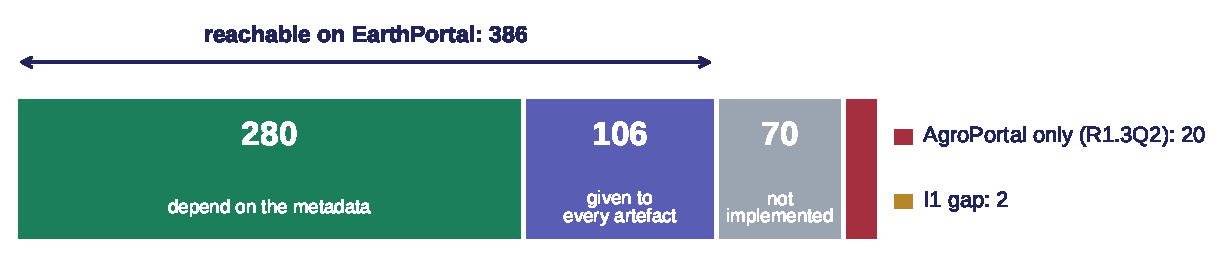
\includegraphics[width=0.92\textwidth]{Figures/fig_478_split.pdf}\\[2pt]
  \begin{columns}[T]
    \begin{column}{0.52\textwidth}
      \small
      Only \textbf{386} points can be earned by an EarthPortal artefact. Beside O'FAIRe's own score,
      we report a \textbf{reachable score}:
      \[
        R(o) = 100 \cdot \frac{S(o)}{386}
      \]
      {\footnotesize It is fair: every removed question gives 0 to everyone, so $S(o)$ only holds reachable points.}
    \end{column}
    \begin{column}{0.44\textwidth}
      \small
      \begin{tabular}{@{}l c c@{}}
        \toprule
        OSO & O'FAIRe $N$ & Reachable $R$\\
        \midrule
        & 76 / 100 & \textbf{94.4\,\%}\\
        \bottomrule
      \end{tabular}\\[6pt]
      \evidence{Split read from the Java code: 12 questions are always given in full (106 points),
      10 are not implemented (70).}
    \end{column}
  \end{columns}
\end{frame}

% =====================================================================================================
\section{The pipeline: five notebooks}

% -----------------------------------------------------------------------------------------------------
\begin{frame}{Overview: one door to the outside world, then pure computation}
  \centering
  \resizebox{\textwidth}{!}{%
  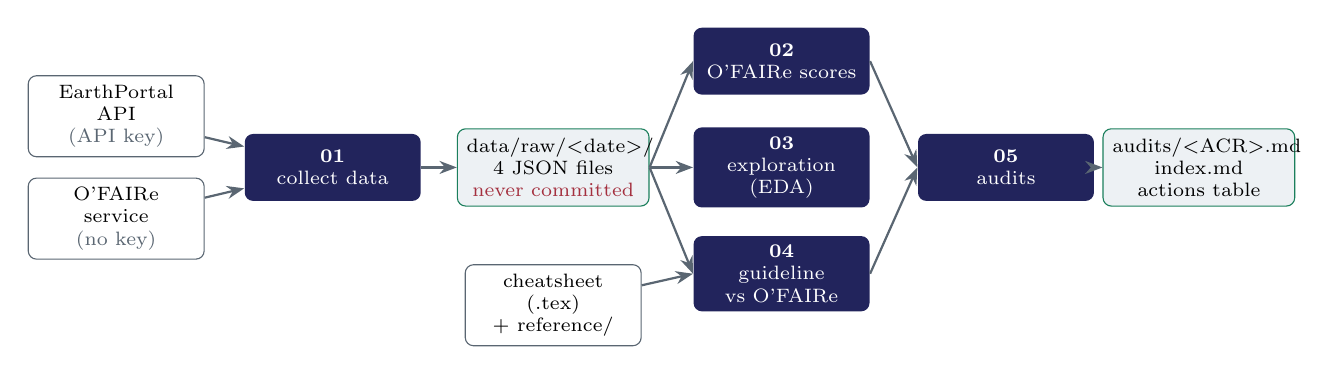
\begin{tikzpicture}[
      font=\scriptsize,
      srcbox/.style={draw=dtgrey, rounded corners=3pt, fill=white, minimum height=0.85cm, text width=2.0cm, align=center},
      nbbox/.style={rounded corners=3pt, fill=dtnavy, text=white, minimum height=0.85cm, text width=2.0cm, align=center},
      outbox/.style={draw=dtteal, rounded corners=3pt, fill=dtband, minimum height=0.85cm, text width=2.2cm, align=center},
      arr/.style={-{Stealth[length=2.2mm]}, dtgrey, line width=0.8pt}]
    \node[srcbox] (api) at (0, 0.65) {EarthPortal API\\{\color{dtgrey}(API key)}};
    \node[srcbox] (of)  at (0,-0.65) {O'FAIRe service\\{\color{dtgrey}(no key)}};
    \node[nbbox]  (n1)  at (2.75, 0) {\textbf{01}\\collect data};
    \node[outbox] (raw) at (5.55, 0) {data/raw/\textless date\textgreater/\\4 JSON files\\{\color{dtred}never committed}};
    \node[nbbox]  (n2)  at (8.45, 1.35) {\textbf{02}\\O'FAIRe scores};
    \node[nbbox]  (n3)  at (8.45, 0) {\textbf{03}\\exploration (EDA)};
    \node[nbbox]  (n4)  at (8.45,-1.35) {\textbf{04}\\guideline vs O'FAIRe};
    \node[srcbox] (cs)  at (5.55,-1.75) {cheatsheet (.tex)\\+ reference/};
    \node[nbbox]  (n5)  at (11.3, 0) {\textbf{05}\\audits};
    \node[outbox] (aud) at (13.75, 0) {audits/\textless ACR\textgreater.md\\index.md\\actions table};
    \draw[arr] (api) -- (n1); \draw[arr] (of) -- (n1); \draw[arr] (n1) -- (raw);
    \draw[arr] (raw.east) -- (n2.west); \draw[arr] (raw) -- (n3); \draw[arr] (raw.east) -- (n4.west);
    \draw[arr] (cs) -- (n4.west);
    \draw[arr] (n2.east) -- (n5.west); \draw[arr] (n4.east) -- (n5.west); \draw[arr] (n5) -- (aud);
  \end{tikzpicture}}
  \vfill
  \small
  \begin{itemize}
    \item \textbf{Only notebook 01 talks to the network.} Notebooks 02 to 05 read a frozen snapshot:
          the same date always gives the same tables, even if EarthPortal changes or is offline.
    \item One \code{config.py} (paths, snapshot date) and one \code{.env} (API key) for all notebooks.
  \end{itemize}
\end{frame}

% -----------------------------------------------------------------------------------------------------
\begin{frame}{Notebook 01: collecting the data}
  \small
  \resizebox{\textwidth}{!}{%
  \begin{tabular}{@{}l l l r@{}}
    \toprule
    \textbf{Part} & \textbf{API call} & \textbf{Saved as} & \textbf{8 Oct}\\
    \midrule
    I. Catalogue & \code{/ontologies} (all fields, views included) & \code{catalogue.json} & 92 entries\\
    II. Portal schema & \code{/submission\_metadata}, \code{/ontology\_metadata} & \code{metadata\_schema.json} & 110 + 20 fields\\
    III. Metadata & \code{/ontologies/<ACR>/latest\_submission} & \code{submissions.json} & 92\\
    IV. O'FAIRe & \code{ofaire/?portal=earthportal}, 10 at a time & \code{ofaire.json} & 92 results\\
    \bottomrule
  \end{tabular}}
  \vspace{8pt}
  \begin{columns}[T]
    \begin{column}{0.48\textwidth}
      \begin{block}{Robust by design}
        \footnotesize
        The key travels in a header, never in a URL; timeouts and three tries before failing;
        answers are saved \textbf{untouched}, in a folder named after the snapshot date.
      \end{block}
    \end{column}
    \begin{column}{0.48\textwidth}
      \begin{alertblock}{Why data/raw/ is never committed}
        \footnotesize
        The raw answers contain contact e-mail addresses, and some pull URLs embed API keys of
        \emph{other} OntoPortal instances.
      \end{alertblock}
    \end{column}
  \end{columns}
\end{frame}

% -----------------------------------------------------------------------------------------------------
\begin{frame}{Notebook 02: from a nested tree to one table}
  \begin{columns}[T]
    \begin{column}{0.50\textwidth}
      \small
      Each O'FAIRe result is a tree: \emph{ontology $\rightarrow$ principle $\rightarrow$
      sub-principle $\rightarrow$ question}. We flatten it into \textbf{one row per ontology}
      (92 $\times$ 68 columns), and we keep \textbf{a missing answer apart from a real 0}:\\[6pt]
      \scriptsize
      \begin{tabular}{@{}l c l@{}}
        \toprule
        Questions & \# & Stored as\\
        \midrule
        Normal & 49 & O'FAIRe's score\\
        Not implemented & 10 & empty (\code{NaN})\\
        F3Q1, always 0 & 1 & empty (\code{NaN})\\
        R1.3Q2, AgroPortal only & 1 & its real 0, out of the 386\\
        \bottomrule
      \end{tabular}
    \end{column}
    \begin{column}{0.47\textwidth}
      \begin{exampleblock}{Three checks against O'FAIRe itself}
        \small
        \begin{enumerate}
          \item the 61 question scores add up to O'FAIRe's total, for \textbf{92 / 92}
          \item $N = \lfloor 100\,S / 478 \rfloor$ holds for \textbf{92 / 92}
          \item $386 = 478 - 90 - 2$ agrees with the definition
        \end{enumerate}
      \end{exampleblock}
      \evidence{The rules for F3Q1 and R1.3Q2 live in \code{reference/ofaire\_known\_issues.csv},
      each with its evidence (Java file, line, commit), not hidden in the code.}
    \end{column}
  \end{columns}
\end{frame}

% -----------------------------------------------------------------------------------------------------
\begin{frame}{Notebook 03: how FAIR is the catalogue today?}
  \begin{columns}[c]
    \begin{column}{0.55\textwidth}
      \centering
      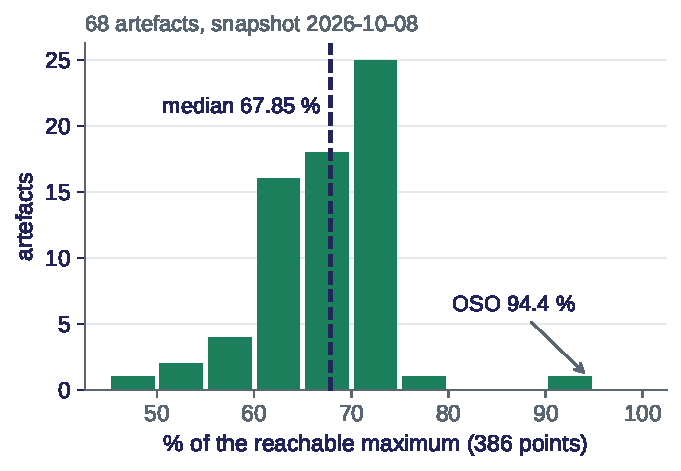
\includegraphics[width=\textwidth]{Figures/fig_reachable_hist.pdf}
    \end{column}
    \begin{column}{0.43\textwidth}
      \small
      \textbf{68 artefacts}, 49 questions they can score on:
      \begin{itemize}
        \item reachable score: median \textbf{67.85\,\%}, from 49.5\,\% (STY) to 94.4\,\% (OSO)
        \item O'FAIRe's own score: median \textbf{54 / 100}
        \item one clear leader; most artefacts between 60 and 75\,\%
      \end{itemize}
      \vspace{2pt}
      \centering
  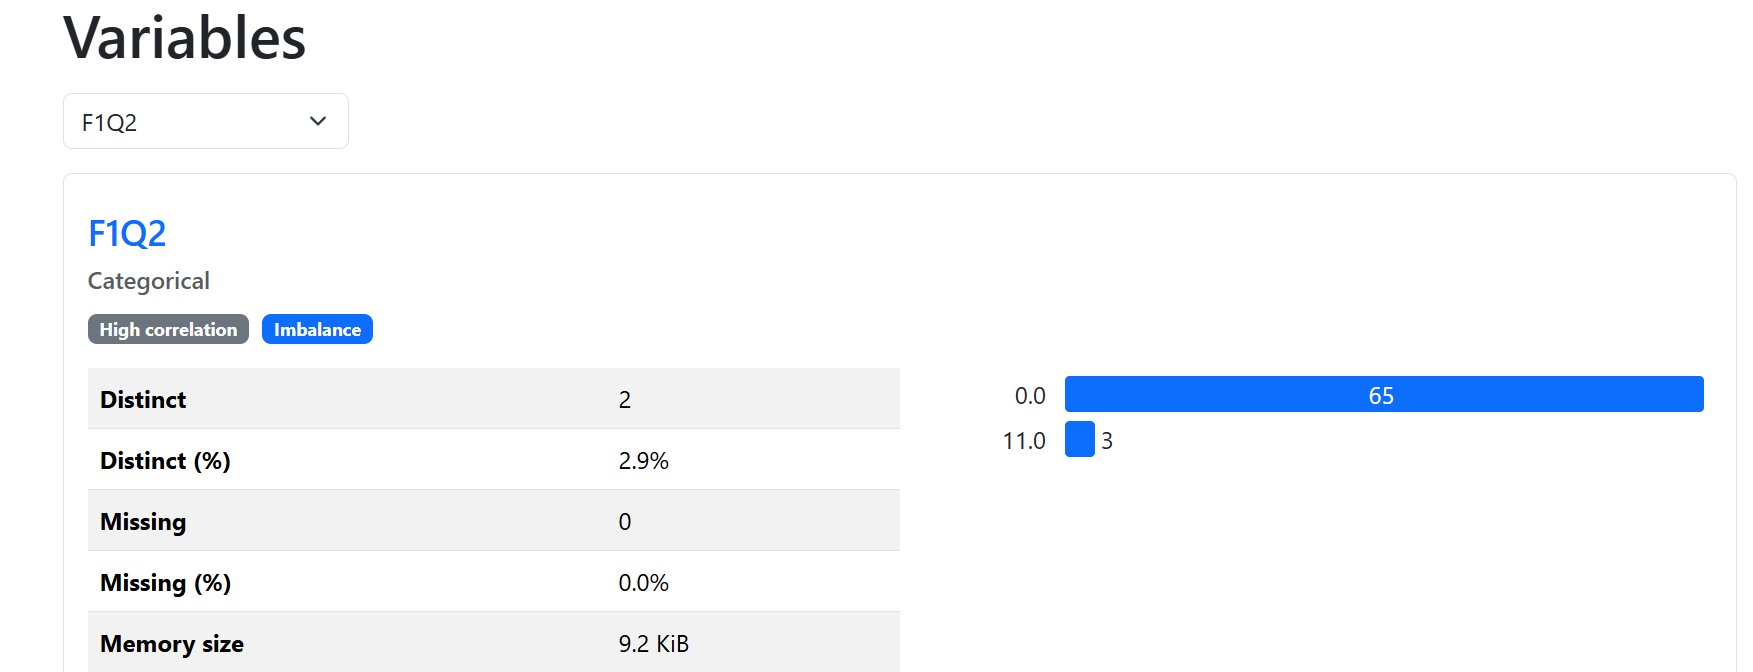
\includegraphics[width=\textwidth]{Figures/F1Q2.png}\\[2pt]
    \end{column}
  \end{columns}
\end{frame}

% -----------------------------------------------------------------------------------------------------
\begin{frame}{Where the catalogue loses most points}
  \begin{columns}[c]
    \begin{column}{0.62\textwidth}
      \centering
      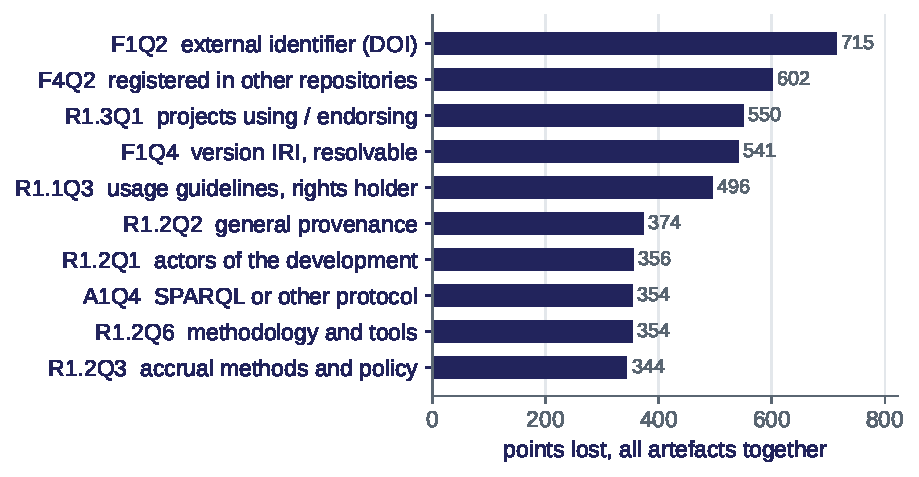
\includegraphics[width=\textwidth]{Figures/fig_lost_points.pdf}
    \end{column}
    \begin{column}{0.36\textwidth}
      \small
      Points lost $= \sum_{o} (m_q - s_q(o))$ over the 68 artefacts.
      \begin{itemize}
        \item \textbf{F1Q2}: 65 artefacts have no external identifier; only a valid
              \textbf{DOI} gives the full 11 points
        \item \textbf{F1Q4}: 59 have no version IRI
        \item \textbf{R1.1Q3}: nobody is at 0, but almost everybody loses part of the 15 points
      \end{itemize}
      \evidence{These first rows are where curation pays most.}
    \end{column}
  \end{columns}
\end{frame}

% -----------------------------------------------------------------------------------------------------
\begin{frame}{Notebook 04, step 1: the guideline becomes machine-readable}
  \small
  \textbf{(a) Read the cheatsheet} (Report 1, \LaTeX) with a regular expression: one table row gives one attribute.\\[4pt]
  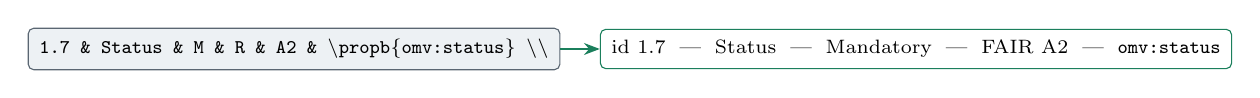
\begin{tikzpicture}[font=\scriptsize]
    \node[draw=dtgrey, fill=dtband, rounded corners=2pt, inner sep=4pt] (a)
      {\texttt{1.7 \& Status \& M \& R \& A2 \& \textbackslash propb\{omv:status\} \textbackslash\textbackslash}};
    \node[right=0.5cm of a, draw=dtteal, rounded corners=2pt, inner sep=4pt] (b)
      {id 1.7 \;|\; Status \;|\; Mandatory \;|\; FAIR A2 \;|\; \texttt{omv:status}};
    \draw[-{Stealth[length=2mm]}, dtteal, line width=0.9pt] (a) -- (b);
  \end{tikzpicture}\\[6pt]
  \textbf{(b) Find where EarthPortal really stores it}: the first rule that works.\\[3pt]
  \begin{columns}[T]
    \begin{column}{0.55\textwidth}
      \scriptsize
      \begin{tabular}{@{}l l r@{}}
        \toprule
        Rule & How & Attributes\\
        \midrule
        \textbf{same} & the guideline property is the portal's own & 72\\
        \textbf{mapping} & in the portal's own \texttt{metadataMappings} & 21\\
        \textbf{manual} & \texttt{reference/manual\_links.csv}, with reasons & 6\\
        \midrule
        & \textbf{linked} & \textbf{99 / 99}\\
        \bottomrule
      \end{tabular}
    \end{column}
    \begin{column}{0.42\textwidth}
      \scriptsize
      \textbf{26} attributes are stored under another property, e.g.\\[2pt]
      \texttt{mod:acronym} $\rightarrow$ \texttt{omv:acronym}\\
      \texttt{dcat:keyword} $\rightarrow$ \texttt{omv:keywords}\\
      \texttt{omv:versionIRI} $\rightarrow$ \texttt{owl:versionIRI}
    \end{column}
  \end{columns}
  \vspace{6pt}
  \textbf{(c) Add what a program needs}: the kind of value the portal expects, its allowed values, and
  \textbf{who can fill it in} (author 86, curator 8, portal 5: a proposal to validate together).\\[3pt]
  $\Rightarrow$ \texttt{mapping/guideline\_profile.csv} and \texttt{.json}: \textbf{the machine-readable guideline}.
\end{frame}

% -----------------------------------------------------------------------------------------------------
\begin{frame}{Notebook 04, step 2: which guideline attributes does each question read?}
  \centering
  \resizebox{\textwidth}{!}{%
  
\begin{tikzpicture}[
      font=\scriptsize,
      box/.style={draw=dtnavy, rounded corners=3pt, fill=white, minimum height=1.0cm, text width=2.15cm, align=center},
      arr/.style={-{Stealth[length=2.2mm]}, dtteal, line width=0.9pt}]
    \node[box, fill=dtnavy, text=white] (q) {O'FAIRe question\\\textbf{F1Q4}\\(9 credits)};
    \node[box, right=0.55cm of q] (p) {property in the result\\\code{owl:versionIRI}};
    \node[box, right=0.55cm of p] (k) {API key\\\code{versionIRI}\\{\tiny from properties.config.json}};
    \node[box, right=0.55cm of k] (f) {portal field\\on the submission};
    \node[box, right=0.55cm of f, fill=dtteal, text=white] (c) {cheatsheet \textbf{1.9}\\Version IRI\\Recommended, author};
    \draw[arr] (q) -- (p); \draw[arr] (p) -- (k); \draw[arr] (k) -- (f); \draw[arr] (f) -- (c);
  \end{tikzpicture}}\\[10pt]
  \begin{columns}[T]
    \begin{column}{0.52\textwidth}
      \begin{alertblock}{A trap we found}
        \small The \code{properties} listed in O'FAIRe's configuration are \textbf{display only}; the
        Java code decides what is read. Where they differ, we follow the code
        (\code{reference/ofaire\_code\_vs\_config.csv}, 4 rows):\\[2pt]
        \scriptsize F2Q1 \textcolor{dtteal}{+}\code{schema:translator};\;
        I3Q3 \textcolor{dtteal}{+}\code{dct:language};\;
        I3Q3 \textcolor{dtred}{$-$}\code{dct:subject};\;
        R1.3Q2 \textcolor{dtteal}{+}\code{omv:acronym}
      \end{alertblock}
    \end{column}
    \begin{column}{0.45\textwidth}
      \small
      \textbf{Result} (\code{mapping/ofaire\_vs\_guideline.csv}):
      \begin{itemize}
        \item 61 questions, \textbf{158} properties read
        \item 33 have no cheatsheet entry: portal metrics and links, object description properties,
              version information, \code{owl:deprecated}
      \end{itemize}
    \end{column}
  \end{columns}
\end{frame}

% -----------------------------------------------------------------------------------------------------
\begin{frame}{Notebook 05: how one file per ontology is written}
  \begin{columns}[T]
    \begin{column}{0.55\textwidth}
      \small
      For each of the 92 entries:
      \begin{enumerate}
        \item \textbf{lost points} on each reachable question: $L_q = m_q - s_q(o)$
        \item \textbf{empty attributes} of the guideline: null, \code{""}, \code{[]}, \code{\{\}}, or an
              agent with nothing but its identifier
        \item each empty attribute $a$ gets a \textbf{share} of the lost points:
              \[ \text{share}(a) = \sum_{q \text{ reads } a} \frac{L_q}{n_q} \]
              {\scriptsize $n_q$: number of empty attributes that $q$ reads. A ranking aid, not a promise of points.}
        \item a \textbf{priority}, then one Markdown file: \code{audits/<ACRONYM>.md}
      \end{enumerate}
    \end{column}
    \begin{column}{0.42\textwidth}
      \begin{block}{Priorities}
        \small
        \begin{tabular}{@{}c l@{}}
          \textbf{P1} & Mandatory\\
          \textbf{P2} & Recommended, costs points\\
          P3 & Recommended only\\
          P4 & Optional, costs points\\
        \end{tabular}
      \end{block}
      \vspace{2pt}
      {\scriptsize Common sense rules: \emph{view of} is asked only of views; \emph{was invalidated by}
      only of retired artefacts.}\\[4pt]
      {\small Also written: \code{audits/index.md} (all entries, best first) and
      \code{data/actions\_<date>.csv} (5\,552 actions).}
    \end{column}
  \end{columns}
\end{frame}

% -----------------------------------------------------------------------------------------------------
\begin{frame}{Example: the audit of OSO, the best artefact}
  \begin{columns}[T]
    \begin{column}{0.56\textwidth}
      \scriptsize
      \textbf{OSO: Observatories of the Seas Ontology}\\
      76 / 100 \,|\, 364.36 / 478 \,|\, \textbf{94.4\,\% of 386} \,|\, rank 1 of 68\\[4pt]
      \begin{tabular}{@{}l r r p{3.6cm}@{}}
        \toprule
        Question & Points & Lost & O'FAIRe says\\
        \midrule
        F4Q2 & 2 / 10 & 8 & registered in 1 ontology repository\\
        A1Q3 & 18 / 24 & 6 & 6 negotiation formats supported\\
        I1Q5 & 0 / 4 & 4 & no other formats declared\\
        R1.2Q2 & 4 / 6 & 2 & 2 provenance properties\\
        I2Q7 & 3.36 / 5 & 1.64 & metadata vocabularies reused\\
        \bottomrule
      \end{tabular}\\[6pt]
      \textbf{Suggested action, by the author:}\\
      {[P2]} Fill \textbf{Is format of} (cheatsheet 6.2, \code{dct:isFormatOf});
      share of the points lost: 4 (I1Q5)
    \end{column}
    \begin{column}{0.41\textwidth}
      \centering
      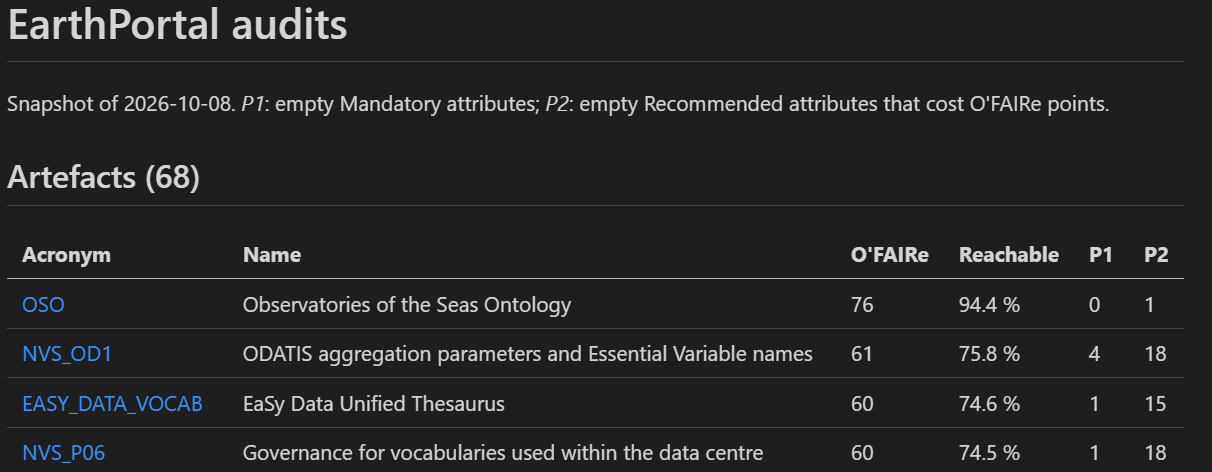
\includegraphics[width=\textwidth]{Figures/INDEX.png}
    \end{column}
  \end{columns}
\end{frame}

% -----------------------------------------------------------------------------------------------------
\begin{frame}{The actions, and who can take them}
  \begin{columns}[c]
    \begin{column}{0.40\textwidth}
      \small
      Artefacts only, priorities 1 and 2:\\[4pt]
      \begin{tabular}{@{}l r r r@{}}
        \toprule
        Who & P1 & P2 & All\\
        \midrule
        author & 89 & 1\,819 & 1\,908\\
        curator & 20 & 61 & 81\\
        portal & 37 & 0 & 37\\
        \midrule
        \textbf{All} & \textbf{146} & \textbf{1\,880} & \textbf{2\,026}\\
        \bottomrule
      \end{tabular}\\[8pt]
      \scriptsize
      \textbf{Location} (pull URL) is empty \emph{by design} when a file is uploaded: should it stay
      Mandatory?\\[2pt]
      \textbf{Portal} rows (CSV dump, download URL, endpoints) point to processing that did not
      produce a value.
    \end{column}
    \begin{column}{0.58\textwidth}
      \centering
      {\small Mandatory attributes most often empty}\\
      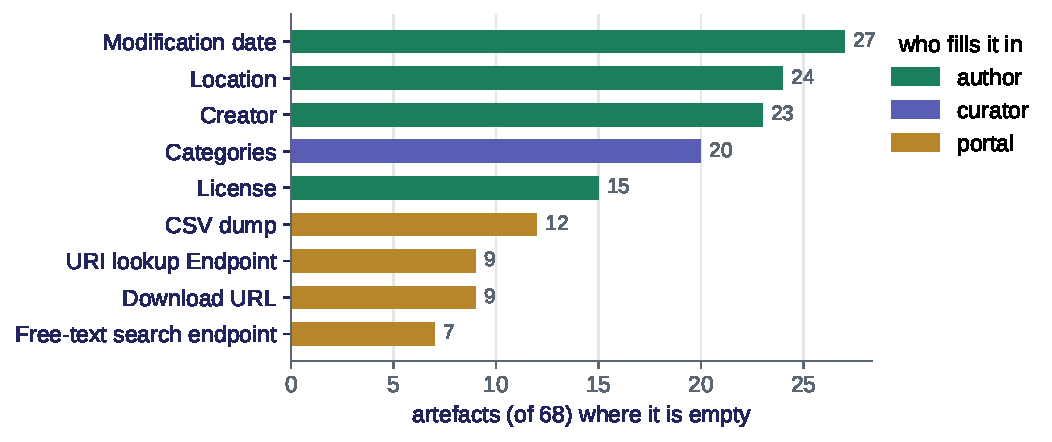
\includegraphics[width=\textwidth]{Figures/fig_mandatory_empty.pdf}
    \end{column}
  \end{columns}
\end{frame}

% =====================================================================================================
\section{What we found}

% -----------------------------------------------------------------------------------------------------
\begin{frame}{Reading O'FAIRe scores correctly: six facts, with evidence}
  \scriptsize
  \renewcommand{\arraystretch}{1.12}
  \begin{tabularx}{\textwidth}{@{}>{\raggedright}p{4.4cm} >{\raggedright}X >{\raggedright\arraybackslash}p{3.3cm}@{}}
    \toprule
    \textbf{Observation} & \textbf{Effect on EarthPortal (8 Oct)} & \textbf{Evidence}\\
    \midrule
    10 questions are not implemented & 0 for 92 / 92 entries, 70 points; always ``cannot be evaluated''
      & setNotResolvable; our check on 5\,612 answers\\
    F3Q1 is a stub; F3Q2 and F3Q3 are always given & F3 reads 21 / 21 for everyone: it carries no information
      & F3.java, line 25\\
    R1.3Q2 rewards hard-coded group names (OBO-FOUNDRY, WHEAT, CROP, INRAE) & 0 / 20 for 92 / 92; none of
      our 15 groups matches & R13.java, lines 50 to 63\\
    I1: maximum 44, but its questions add up to 42 & no artefact can reach 100\,\% on I1
      & I1Q1 ladder changed in commit a170016 (2022)\\
    I2Q7 = 5 $\times$ average vocabulary weight; highest weight 0.75 & capped at 3.75 / 5; the MOD 3.0
      namespace (w3id.org/mod\#) earns nothing & I2.java, line 124; metadata.voc.config.json\\
    EarthPortal is not in the known catalogues & F4Q1 / F4Q2 start one rung lower than on AgroPortal;
      F4Q2 is our 2nd largest loss & catalogs.config.json\\
    \bottomrule
  \end{tabularx}
  \vfill
  \evidence{Source read: github.com/agroportal/fairness, commit 24def6b (4 June 2026). All checks are
  reproducible from the notebooks and from \texttt{reference/}.}
\end{frame}

% -----------------------------------------------------------------------------------------------------
\begin{frame}{Four more things a curator should know}
  \begin{columns}[T]
    \begin{column}{0.48\textwidth}
      \begin{block}{Presence, not correctness}
        \small A field counts as filled when it is not empty: \code{"N/A"} or \code{"to be done"} pass.
        Our audits share this limit for now.
      \end{block}
      \begin{block}{Truncated percentage}
        \small $N = \lfloor\,\cdot\,\rfloor$, not rounded: OSO's 76.2 is shown as 76.
      \end{block}
    \end{column}
    \begin{column}{0.48\textwidth}
      \begin{alertblock}{Scores are not dated}
        \small In portal mode, O'FAIRe serves cached results, with no date or submission id. On 17 September,
        OSO's panel showed other values (version IRI, DOI, counts) than its page.
      \end{alertblock}
    \end{column}
  \end{columns}
  \vfill
  \evidence{We do not know which O'FAIRe commit runs on the EarthPortal server, nor how often its cache is refreshed.}
\end{frame}

% -----------------------------------------------------------------------------------------------------
\begin{frame}{Observations on the catalogue itself}
  \small
  \begin{itemize}
    \item \textbf{5 metadata-only records look like tests}: \code{TEST}, \code{HG} (``Hello Go''),
          \code{SW}, \code{HIG} (``HI Go''), \code{GTD} (``GO TO DO''). Remove them?
    \item \textbf{Views of OSO}: \code{OSO-DCAT}, \code{OSO-VOID} and \code{OSO-SHACL} are now declared as views,
          which solves our earlier finding that \code{OSO-DCAT} shared OSO's URI.
    \item \textbf{5 pull URLs} embed an API key of another OntoPortal instance (masked in all our outputs).
  \end{itemize}
  \vfill
  \evidence{The last three points come from the snapshot of 28 September 2026 and must be checked again on the current one.}
\end{frame}

% -----------------------------------------------------------------------------------------------------
\begin{frame}{Questions I would like to discuss}
  \begin{columns}[T]
    \begin{column}{0.50\textwidth}
      \begin{block}{For the EarthPortal team}
        \small
        \begin{enumerate}
          \item Is the split \textbf{author / curator / portal} right?
          \item Should \textbf{Location} stay Mandatory for uploaded files?
          \item Who contacts the owners: authors (audits), and portals whose \textbf{keys} are exposed?
          \item Can the \textbf{test records} be removed?
        \end{enumerate}
      \end{block}
    \end{column}
    \begin{column}{0.46\textwidth}
      \begin{block}{For the O'FAIRe team}
        \small
        \begin{enumerate}
          \setcounter{enumi}{4}
          \item Which \textbf{commit} runs on EarthPortal, and how often is the \textbf{cache} refreshed?
          \item Could EarthPortal be listed in \code{catalogs.config.json}?
          \item Where should our evidence go: GitHub issues on \code{agroportal/fairness}?
        \end{enumerate}
      \end{block}
    \end{column}
  \end{columns}
\end{frame}

% =====================================================================================================
\section{Environment and next steps}

% -----------------------------------------------------------------------------------------------------
\begin{frame}{Environment: open and reproducible}
  \begin{columns}[T]
    \begin{column}{0.30\textwidth}
      \centering
      \qrcode[height=2.5cm]{https://github.com/EarthPortal/SA_Management}\\[4pt]
      {\scriptsize\href{https://github.com/EarthPortal/SA_Management}{github.com/EarthPortal/SA\_Management}}\\[6pt]
      \raggedright\scriptsize
      \textbf{docs/}: reports (\LaTeX, PDF)\\
      \textbf{earthportal\_sa\_audit/}: notebooks, tables, audits\\
      one \texttt{.env}, one \texttt{requirements.txt}; MIT licence
    \end{column}
    \begin{column}{0.67\textwidth}
      \scriptsize
      \textbf{The notebooks run on an HPC node of Area Science Park (Trieste)}\\[3pt]
      \begin{tabular}{@{}l l@{}}
        \toprule
        Node & epyc006.hpc.rd.areasciencepark.it, partition EPYC (Slurm)\\
        CPU & 2 $\times$ AMD EPYC 7H12, 64 cores each (128 cores)\\
        Memory & 503 GiB, no GPU\\
        OS & Fedora Linux 41\\
        My session & Slurm job of 12 CPUs, 48 GB, 2 hours; VS Code through a tunnel\\
        Python & 3.13.9 in a virtual environment; pandas 2.3.3, fg-data-profiling 4.20.0\\
        \bottomrule
      \end{tabular}\\[6pt]
      \textbf{Reports} are written in \LaTeX\ on my PC (WSL Ubuntu, TeX Live, VS Code);
      the same git identity is used on both machines.
    \end{column}
  \end{columns}
\end{frame}

% -----------------------------------------------------------------------------------------------------
\begin{frame}{What comes next}
  \begin{columns}[T]
    \begin{column}{0.32\textwidth}
      \begin{block}{Next weeks}
        \small
        \begin{itemize}
          \item validate \emph{who fixes} and the priorities with you
          \item re-check the catalogue observations on today's snapshot
          \item first contacts with authors, starting with P1
        \end{itemize}
      \end{block}
    \end{column}
    \begin{column}{0.32\textwidth}
      \begin{block}{Then}
        \small
        \begin{itemize}
          \item validation rules in the machine-readable guideline (value checks, not only presence)
          \item scheduled snapshots: a history of the scores
          \item compare with \textbf{FOOPS!}
        \end{itemize}
      \end{block}
    \end{column}
    \begin{column}{0.32\textwidth}
      \begin{exampleblock}{The goal}
        \small A curation pipeline that \textbf{proposes} changes, which a curator
        \textbf{validates} in an admin interface (possibly with AI support).
      \end{exampleblock}
    \end{column}
  \end{columns}
\end{frame}

% -----------------------------------------------------------------------------------------------------
{
\setbeamercolor{background canvas}{bg=dtnavy}
\setbeamercolor{normal text}{fg=white}
\usebeamercolor[fg]{normal text}
\begin{frame}[plain]
  \centering
  \vspace{0.6cm}
  {\Large\bfseries Thank you for your attention}\\[8pt]
  {\large Merci beaucoup de votre attention}\quad\textcolor{dtband}{$\cdot$}\quad
  {\large Grazie mille}\quad\textcolor{dtband}{$\cdot$}\quad
  {\large Aksante saana}\\[1.1cm]
  {\itshape ``All models are wrong, but some are useful.''}\\[2pt]
  {\small George E.\ P.\ Box}\\[0.6cm]
  {\itshape ``Big goals, small steps.''}\\[1.0cm]
  {\small\href{https://github.com/EarthPortal/SA_Management}{github.com/EarthPortal/SA\_Management}}
\end{frame}
}

% =====================================================================================================
\appendix

% -----------------------------------------------------------------------------------------------------
\begin{frame}{Backup: the ten questions O'FAIRe does not implement}
  \scriptsize
  \begin{tabularx}{\textwidth}{@{}l r X@{}}
    \toprule
    Question & Max & Text\\
    \midrule
    F4Q3 & 8 & Are the ontology libraries or repositories properly indexed by Web search engines?\\
    I2Q3 & 3 & If yes, does it include the minimum information for those terms?\\
    I2Q5 & 7 & If yes, are those alignments well represented and to unambiguous entities? \dots\\
    I3Q1 & 20 & Does an ontology provide qualified cross-references to external resources/databases?\\
    I3Q2 & 6 & If yes, are those cross-references well represented and to unambiguous entities?\\
    R1Q3 & 7 & How much of the ontology objects are described with labels?\\
    R1Q4 & 6 & How much of the ontology objects are defined using a text description?\\
    R1Q5 & 6 & How much ontology objects are defined using a property restriction or an equivalent class?\\
    R1Q6 & 5 & How much of the ontology objects provide provenance information with annotation properties?\\
    R1.2Q5 & 2 & Are the ontology latest changes documented?\\
    \midrule
    \textbf{Total} & \textbf{70} & Every answer: ``This question cannot be evaluated in the repository at this time.''\\
    \bottomrule
  \end{tabularx}
\end{frame}

% -----------------------------------------------------------------------------------------------------
\begin{frame}{Backup: the snapshots so far}
  \small
  \begin{tabular}{@{}l c c c c c@{}}
    \toprule
    Snapshot & Entries & Artefacts & Views & Metadata-only & OSO (reachable)\\
    \midrule
    28 Sept 2026 & 91 & 70 & 16 & 5 & 93.9\,\%\\
    2 Oct 2026 & 92 & 71 & 16 & 5 & 93.9\,\%\\
    6 Oct 2026 & 92 & 71 & 16 & 5 & 94.4\,\%\\
    8 Oct 2026 & 92 & 68 & 19 & 5 & 94.4\,\%\\
    \bottomrule
  \end{tabular}\\[10pt]
  \begin{itemize}
    \item by 2 October: \code{SCHEMA-ORG} (Schema.org) appears as an artefact
    \item between 6 and 8 October: \code{SCHEMA-ORG} is no longer public; \code{OSO-SHACL} appears as a
          view of OSO; \code{OSO-DCAT} and \code{OSO-VOID} become views of OSO
    \item median reachable score of the artefacts: 67.6\,\% (2 and 6 Oct), 67.85\,\% (8 Oct)
  \end{itemize}
  \vfill
  \evidence{Tables in \code{earthportal\_sa\_audit/data/}, one set per snapshot date.}
\end{frame}

\end{document}
